\chapter{Heritability of Schizophrenia}

\section{Introduction}
% There is a large developmental thingy in schizophrenia
% So will genes co-express in the brain during brain development 
% be enriched with the heritability?
% Need to talk about BrainSpan
% Need to talk about WGCNA
% Mention about RPKM
\citet{Bulik-Sullivan2015,Finucane2015,Bulik-Sullivan2015a} have performed a series of comprehensive studies on the heritability of \glng{scz}.
 
Apply Heritability estimation to the schizophrenia data.
The genetic correlation and partitioning of heritability
No one worked on linking schizophrenia with brain development directly?
\section{Heritability Estimation}
This will be a very simple section, focused on how to perform the heritability estimation on \acrfull{scz}.
Should also tokenize the heritability into subcategories (e.g. immune, neuron, etc)
%Should not put too much weight into it, otherwise it will be a direct copy of LDSC. Won't really add much power. 


\subsection{Methodology}
\subsection{Result}
\section{Brain development and Schizophrenia}
\sectionmark{Brain development}
Here we will perform the WGCNA and brain development network.
Seeing how the whether if any brain development network were enriched with SNPs that explain the variance of phenotype
%Instead, we should put most focus here as no one has done it before
%Also descript brainspan here
\subsection{Methodology}
\subsubsection{Sample Quality Controls}
Developmental transcriptome data were obtained from BrainSpan (\url{http://www.brainspan.org/}).
A total of 56 individual with different ages were provided. 
Considering the age of onset of \glng{scz}, we selected an age cut off of 30 years old. 
Any individual older than 30 years old were excluded from the analysis.
An individual can have more than one regions sequenced, thus there were a total of 524 RNA Sequencing data available.
We only select samples with dissection score $>3$ and an \gls{rin}$\ge7$.
This gave us a total of 421 brain expression data, subdivided into 21 regions according to the BrainSpan meta data.

A challenge in trying to build co-expression gene networks using the BrainSpan samples were the relatively small sample size.
As for some age, there were only as little as 1 individual, we cannot build a separate gene co-expression networks for each age. 
Rather, we can only build a gene co-expression networks containing genes that were co-expressed in all sample age. 
By combining samples from different age together, we will have adequate sample size for the network construction.
However, another problem arise when merging all samples together was the possibility of over-representing age groups with more individual. 
Thus, when more than 1 samples were available for a particular age group, we will only use the sample with the best quality.
Samples with higher dissection score were always preferred as they should better represent their region. 
In situation where there were multiple samples with the same dissection score, we select sample with a higher \gls{rin} value, which indicate a better RNA quality.
Finally, for any region, we require at least 10 samples after the quality control were performed such that we will have a sufficient number of sample for network construction.
In the end, 16 brain regions each with 14-21 samples were selected for gene co-expression network construction.

%Studies suggested Hippocampus\citep{Velakoulis2006,Nugent2007}, Amygdala and Striatum\citep{Simpson2010} are brain regions involved in the etiology of schizophrenia. 
%Therefore, we focus on building the gene co-expression network of hippocampus, amygdala and striatum in this study
%RNA Sequencing data of the brain regions were obtained from BrainSpan and undergo a series of quality control before the construction of the network. 

\subsubsection{Normalization of data}
The RNA Sequencing data were represented as \gls{rpkm} values.
The \gls{rpkm} normalization were used such that count data from different samples can be comparable without worrying the difference in sequencing depth. 
Genes with a low \gls{rpkm} were usually a result from technical or biological noise\citep{Hart2013}.
Thus to reduce noise in the final model, genes with a mean \gls{rpkm} $< 1$ in all samples were discarded. 
The \gls{rpkm} were then log$_2$ transformed as instructed by the manual of \gls{wgcna}\citep{Langfelder2008}.

As there are insufficient samples for the construction of gene co-expression network for individual sample age, we try to construct networks with genes co-expressed through all sample stage. 
This is achieved by taking the standardized log$_2$ \gls{rpkm} across sample age such that all genes has a mean of 0 and standard deviation of 1.

\begin{table}
	\centering
	\caption[Region information for network construction]{Region information for network construction.
		The soft-threshold was picked based on \citet{Langfelder2008}.
		When multiple saturation level were found, the first soft-threshold with scale free $R^2 \ge 0.8$ were selected unless the expected median connectivity was lower than 30 (default minimum network size).
		The reason for the restriction placed on the expected median connectivity was that we do not want to construct very small networks, which were likely to be a result of noise.
	}
	\begin{tabular}{p{9cm}p{1.5cm}p{2cm}p{1.5cm}}
		\toprule
		Region & Acronym & Number of Samples & Soft-Threshold \\
		\midrule
		 Primary auditory cortex (core) & A1C & 16 & 16 \\%
		 Amygdaloid complex & AMY & 15 & 14 \\%
		 Cerebellar cortex & CBC & 18 & 15 \\
		 Dorsolateral prefrontal cortex & DFC & 21 & 26\\
		 Hippocampus (hippocampal formation) & HIP & 17 & 16 \\
		 Posteroventral (inferior) parietal cortex & IPC & 18 & 9 \\
		 Inferolateral temporal cortex (area TEv, area 20) & ITC & 16 & 17 \\ %
		 Primary motor cortex (area M1, area 4) & M1C & 14 & 10  \\ 
		 Mediodorsal nucleus of thalamus & MD & 14 & 22  \\
		 anterior(rostral) cingulate(medial prefrontal) cortex & MFC & 17 & 12 \\
		 Orbital frontal cortex & OFC & 16 & 15 \\
		 Primary somatosensory cortex (area S1, areas 3,1,2) & S1C & 14 & 16 \\
		 Posterior (caudal) superior temporal cortex (area 22c) & STC & 21 & 12 \\
		 Striatum & STR & 16 & 16 \\
		 Primary visual cortex (striate cortex, area V1/17) & V1C & 18 & 20 \\
		 Ventrolateral prefrontal cortex & VFC & 19 & 27\\
		\bottomrule
		\label{tab:regionSample}
	\end{tabular}
\end{table}
\subsubsection{Network Construction}
\gls{wgcna} (ver 1.47) were used for the construction of gene co-expression network\citep{Langfelder2008}. 
The \emph{blockwiseModules} function, using Biweight Midcorrelation for the correlation matrix and a restriction of minimum network size of 30 were used.
During the construction of gene co-expression network using \gls{wgcna}, one need to select a soft-power threshold such that the constructed network should be \emph{scale-free}.
Based on \citet{Zhang2005}, we select the first $R^2$ that was saturated with $R^2>0.7$. 

%\begin{figure}
%	\caption[Soft-power threshold selection]{Soft-power threshold selection. A soft-power of 13 were selected as it is the first threshold value having $R^2 > 0.8$ (0.817) and where the $R^2$ is saturated.}
%	\centering
%	\scalebox{.8}{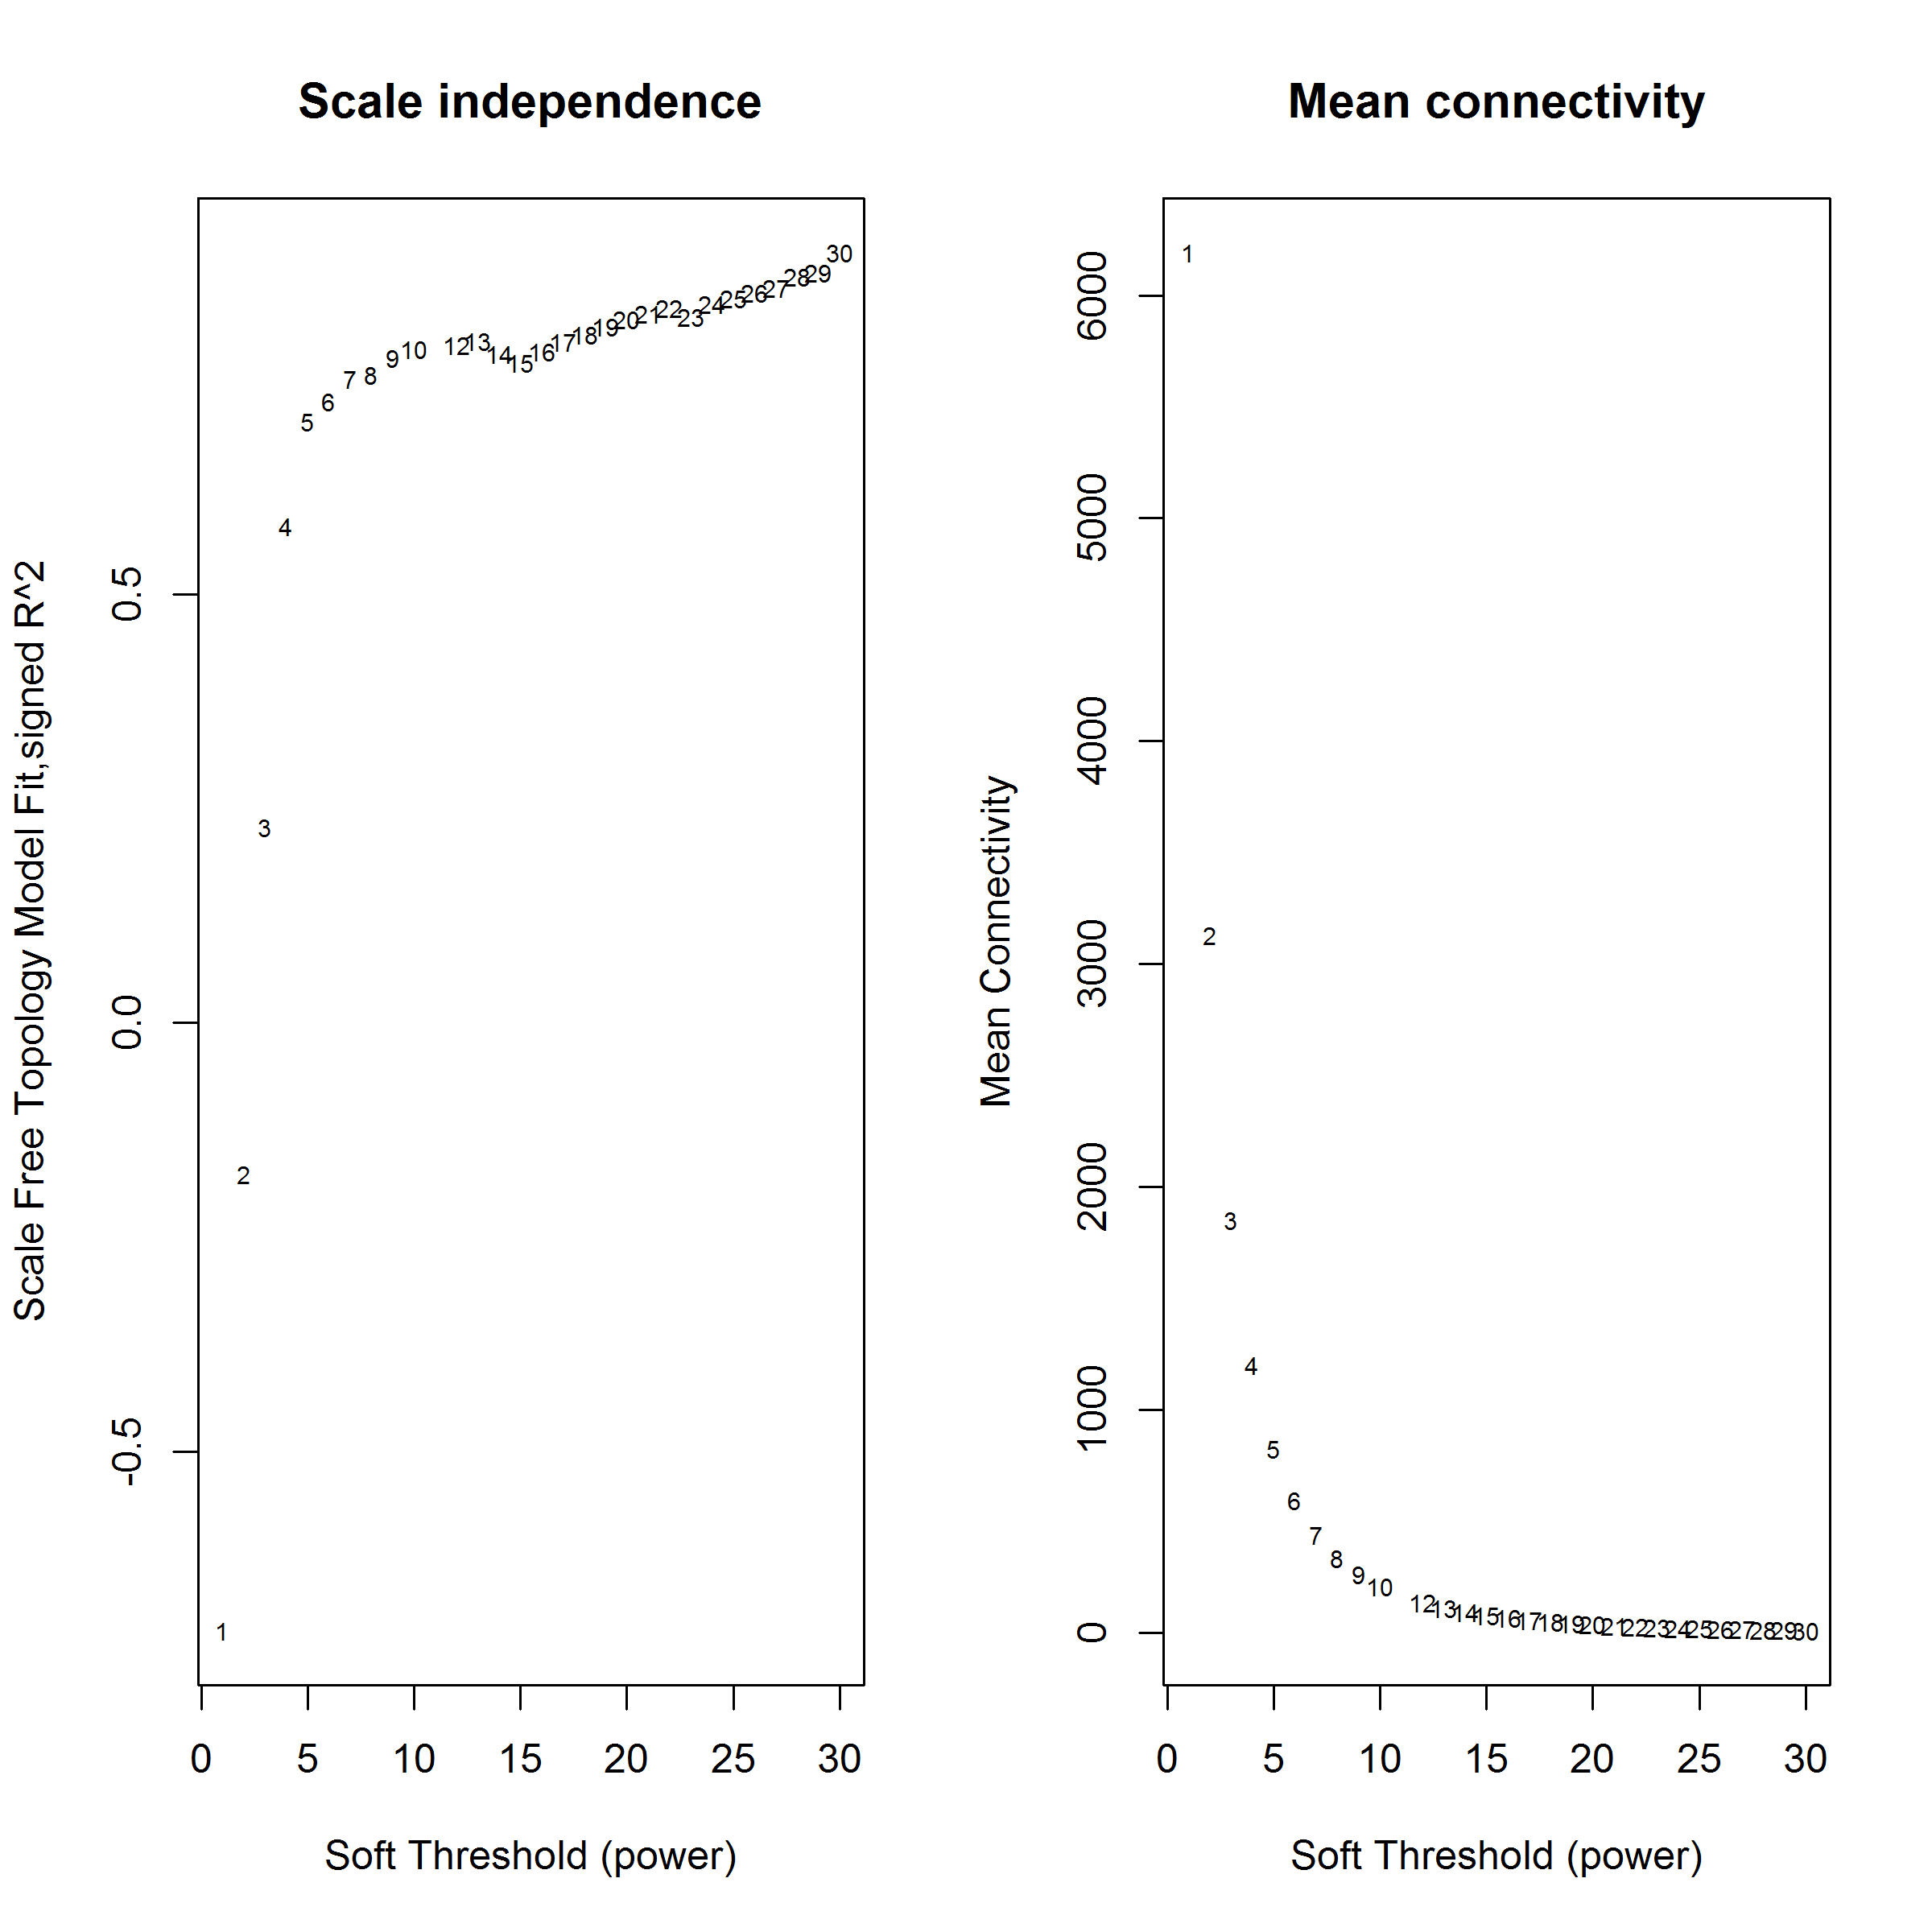
\includegraphics{figure/SoftpowerThreshold.png}}
%	\label{fig:softpowerThreshold}
%\end{figure}

\subsubsection{Expression correlation with Age}
The co-expression network constructed with the standardized gene expression value will contains genes that co-express in all sample age.
However, this does not necessary suggest the expression of these genes are correlated with the sample age.
To identify gene co-expression networks with expressions correlated with the sample age, we performed a correlation analysis between the module eigen-genes and the sample age. 
Network eigen-genes were calculated as the first \gls{pc} of expressions of the genes within individual networks using the \emph{moduleEigengenes} function from \gls{wgcna}. 
Age were represented as month from conception such that 8 post-conception week will be represented as 2; 4 months will be represented as 10 and 12 years will be represented as 154 etc. 
Finally, correlation between age and network eigen-gene expression were calculated pearson correlation.

\subsubsection{Functional Annotation}
\gls{GO} based enrichment analysis of the significant module was performed using GOrilla\citep{Eden2009}.
Genes within the networks were provide as the target gene lists and all the genes passed quality controls were used as the background gene list.
As \gls{GO} terms tends to be redundant and overlaps with each other, it will aid the interpretation of \gls{GO} results based by clustering and reducing the \gls{GO} terms based on their similarity. 
Thus, \gls{GO} enrichment results were summerized by REViGO\citep{Supek2011} and significant representative \gls{GO} terms were obtained.

\subsubsection{Associate Co-expression network with \glsentryshort{pgc} schizophrenia data}
The co-expression networks were built from normal samples and should not be representative of the brain expression pattern in schizophrenia patients.
it is however interesting to see if the co-expression networks were disrupted in schizophrenia patient.
To test whether if the gene co-expression networks contain genes that are jointly associated with schizophrenia, we first use \gls{MAGMA}\citep{DeLeeuw2015}(version v1.03) to compute the gene-base p-value from the \gls{SNP} wise p-value obtained from \gls{pgc}. 
Gene-set enrichment analysis were then performed on networks that were significantly correlated with developmental age. 
As we were only interested in whether if the genes within the networks were jointly associated with schizophrenia, we only focus on the result of the self-contained gene set analysis and ignore the result from competitive analysis.

\subsubsection{Partitioning of Heritability}

\subsection{Result}
\subsubsection{Co-Expression Network}
A total of 35 networks were constructed based on the hippocampus samples with a mean network size of 421.6.
On the other hand, 28 networks were constructed for amygdala with mean network size of 591.86.
Finally, 25 networks with mean size of 494.52 were constructed from the striatum samples.

Of the all the networks constructed, only one network from hippocampus(\cref{tab:hipModSig}) and three networks from amygdala(\cref{tab:amyModSig}) were significantly correlated with sample age after bonferroni correction threshold (p-value $<0.00143$ for hippocampus, p-value $<0.00179$ for amygdala and p-value $<0.002$ for striatum) .
\begin{table}
	\centering
	\caption[Correlation of sample age with the module eigen gene]{Correlation of sample age with the module eigen gene. 
		Module eigen-gene was defined as the first \gls{pc} of genes within the module. 
		After correcting for multiple testing, only the black module was considered as significantly correlated with the sample age.}
	\subfloat[Hippocampus]{
		\begin{tabular}{rrr}
			\toprule
			& Correlation & Pvalue \\
			\midrule
			black & 0.804653 & 0.000171 \\
			blue  & -0.61648 & 0.010981 \\
			red   & -0.60207 & 0.013595 \\
			darkred & -0.59137 & 0.015833 \\
			greenyellow & -0.56995 & 0.021168 \\
			yellow & 0.567828 & 0.021763 \\
			darkgrey & -0.55246 & 0.026474 \\
			saddlebrown & -0.52983 & 0.034783 \\
			turquoise & -0.51371 & 0.041809 \\
			purple & -0.46788 & 0.067606 \\
			darkolivegreen & -0.41272 & 0.112122 \\
			sienna3 & -0.39535 & 0.129604 \\
			darkturquoise & 0.386541 & 0.139154 \\
			darkorange & 0.384966 & 0.140912 \\
			darkmagenta & 0.375586 & 0.151688 \\
			brown & 0.366095 & 0.163144 \\
			tan   & -0.36522 & 0.164229 \\
			pink  & 0.348979 & 0.18524 \\
			magenta & -0.32559 & 0.218473 \\
			midnightblue & -0.29168 & 0.273014 \\
			lightgreen & 0.289921 & 0.276056 \\
			paleturquoise & -0.28045 & 0.29276 \\
			white & 0.27727 & 0.29849 \\
			orange & 0.19607 & 0.466754 \\
			steelblue & 0.17355 & 0.520357 \\
			skyblue & 0.145869 & 0.589857 \\
			lightyellow & -0.11665 & 0.667028 \\
			green & -0.09882 & 0.715786 \\
			violet & -0.08757 & 0.747076 \\
			lightcyan & -0.0656 & 0.809257 \\
			cyan  & -0.06441 & 0.812661 \\
			darkgreen & -0.03914 & 0.885582 \\
			salmon & 0.038727 & 0.886769 \\
			royalblue & -0.03785 & 0.889314 \\
			grey60 & 0.03119 & 0.908709 \\
			\bottomrule
			\label{tab:hipModSig}%
		\end{tabular}%
	}
	\qquad%
	\subfloat[Amygdala]{
		\begin{tabular}{rrr}
			\toprule
			& Correlation & P-value \\
			\midrule
			tan   & 0.849999 & $7.96\times 10^{-6}$ \\
			yellow & -0.757 & $2.76\times 10^{-4}$ \\
			pink  & -0.68541 & $1.69\times 10^{-3}$ \\
			greenyellow & -0.67831 & $1.97\times 10^{-3}$ \\
			red   & -0.64532 & $3.83\times 10^{-3}$ \\
			turquoise & -0.59771 & $8.80\times 10^{-3}$ \\
			lightyellow & -0.56347 & 0.0149 \\
			brown & 0.548516 & 0.0184 \\
			darkgreen & -0.46366 & 0.0526 \\
			blue  & -0.4604 & 0.0545 \\
			purple & -0.44182 & 0.0664 \\
			darkgrey & -0.39065 & 0.109 \\
			orange & -0.36966 & 0.131 \\
			white & 0.28737 & 0.248 \\
			darkred & 0.283247 & 0.255 \\
			black & 0.271383 & 0.276 \\
			salmon & -0.24203 & 0.333 \\
			skyblue & 0.207071 & 0.410 \\
			cyan  & 0.18778 & 0.456 \\
			lightgreen & 0.166495 & 0.509 \\
			grey60 & 0.15156 & 0.548 \\
			midnightblue & 0.136078 & 0.590 \\
			magenta & -0.13459 & 0.594 \\
			darkturquoise & 0.129954 & 0.607 \\
			lightcyan & 0.090241 & 0.722 \\
			darkorange & -0.05166 & 0.839 \\
			green & -0.04745 & 0.852 \\
			royalblue & 0.020456 & 0.936 \\
			\bottomrule
			\label{tab:amyModSig}%
		\end{tabular}%
	}
\end{table}

By plotting the mean expression of each network against the sample age, one can inspect how the dynamic of the network changes across different developmental stage.
Thus, mean expression of all the genes within the significant networks were calculated for all amygdala (n=33) and hippocampus (n=32) samples from BrainSpan.
The mean \gls{rpkm} values were then log$_2$ transformed and plot against the sample age where a line of bests fit was calculated using the \emph{stat\_smooth} with the loess function from R package \emph{ggplot2}(version 1.0.1). (\cref{fig:allMod}).

The expression pattern observed were intriguing where there both the ``black''(\cref{fig:blackMod}) and ``tan'' (\cref{fig:tanMod}) networks have mean gene expression level increase as development progress and reaches its peak at around late adolescence ($\approx 18-21$), concurring with the onset age of schizophrenia.
Similarly, an inverse pattern were observed with the ``yellow'' network where its mean expression was highest during fetal development and drop steadily to its lowest around late adolescence and increase again afterwards(\cref{fig:yellowMod}).

The expression pattern of the ``black'' and ``tan'' networks are of particular interest as they follow the inverted ``U'' shape trajectory of the grey matter volumn observed in previous studies\citep{Gogtay2011}, suggest that they might have a role in mediating brain development. 
\begin{figure}
	\caption[Mean Gene Expression across developmental age]{Mean Gene Experssion across developmental age.
		Mean \gls{rpkm} values of genes in the significant modules were plot with respect to the sample age.
		A loess smoothing curve was also plotted. 
		%Might want to talk somemore about it
	}
	\centering
	\subfloat[``Black'' Network from Hippocampus]{
		\scalebox{.4}{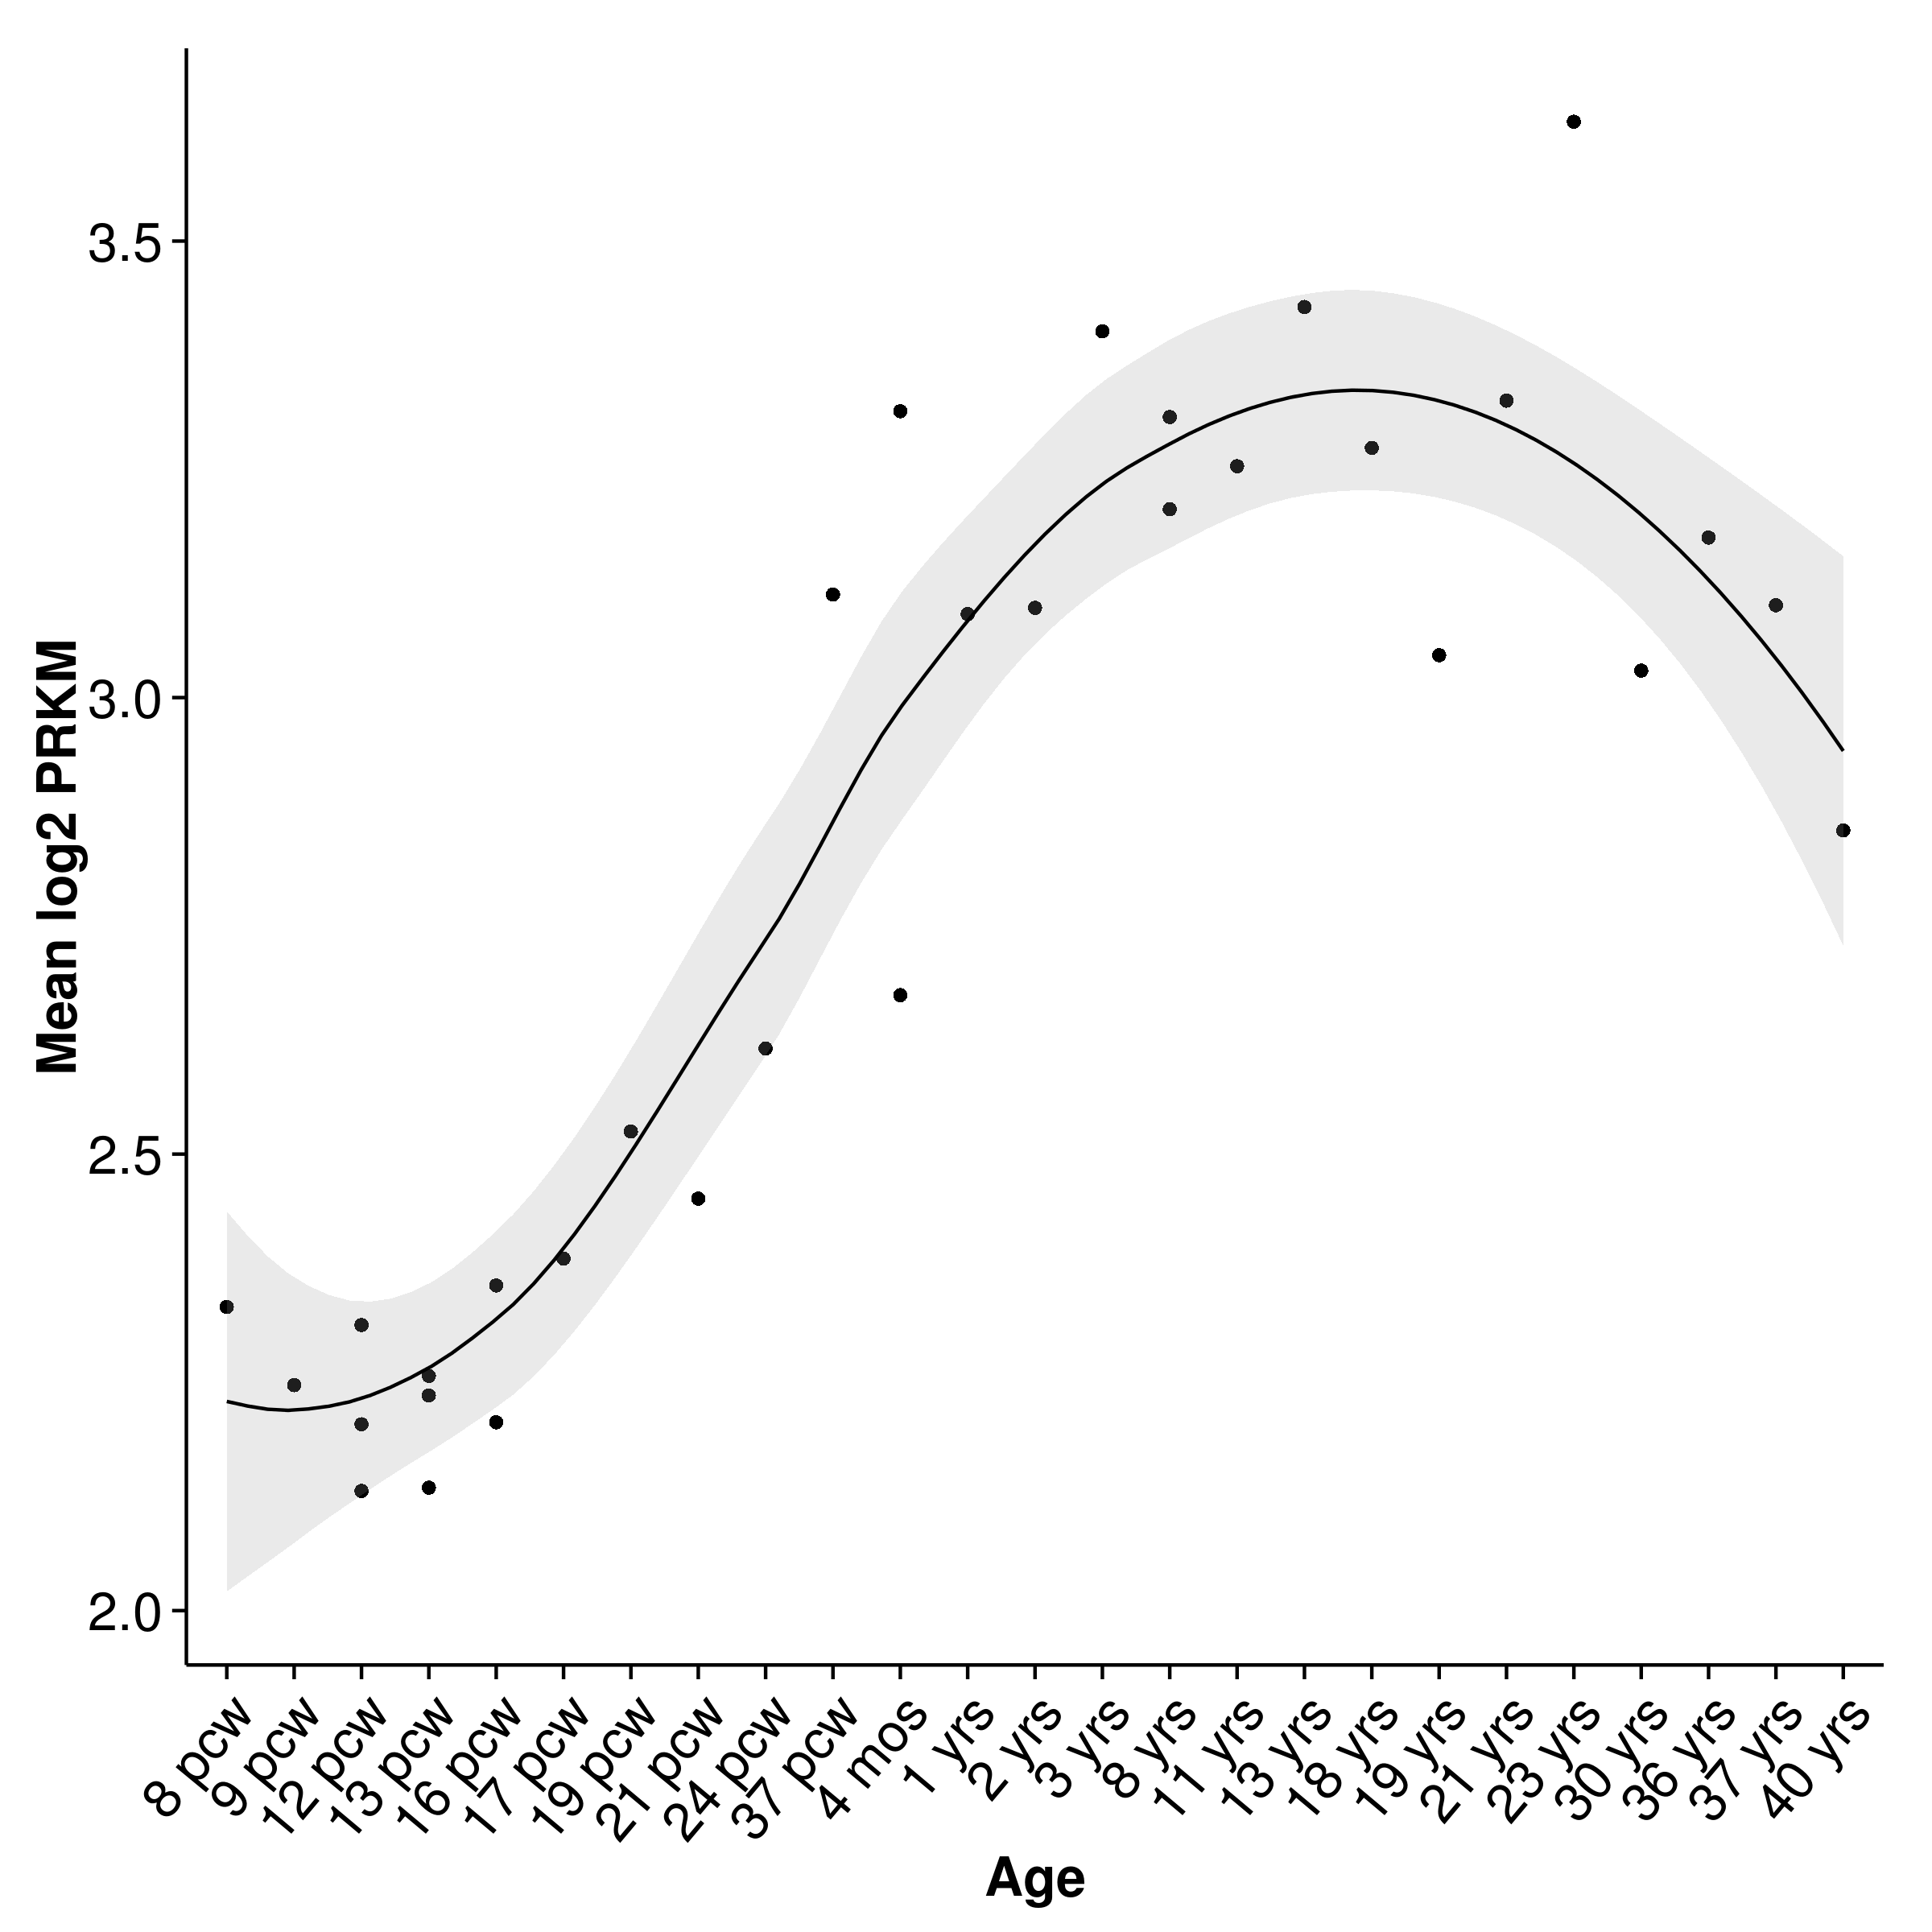
\includegraphics{figure/network/hip_network.png}}
		\label{fig:blackMod}
	}
	\subfloat[``Tan'' Network from Amygdala]{
		\scalebox{.4}{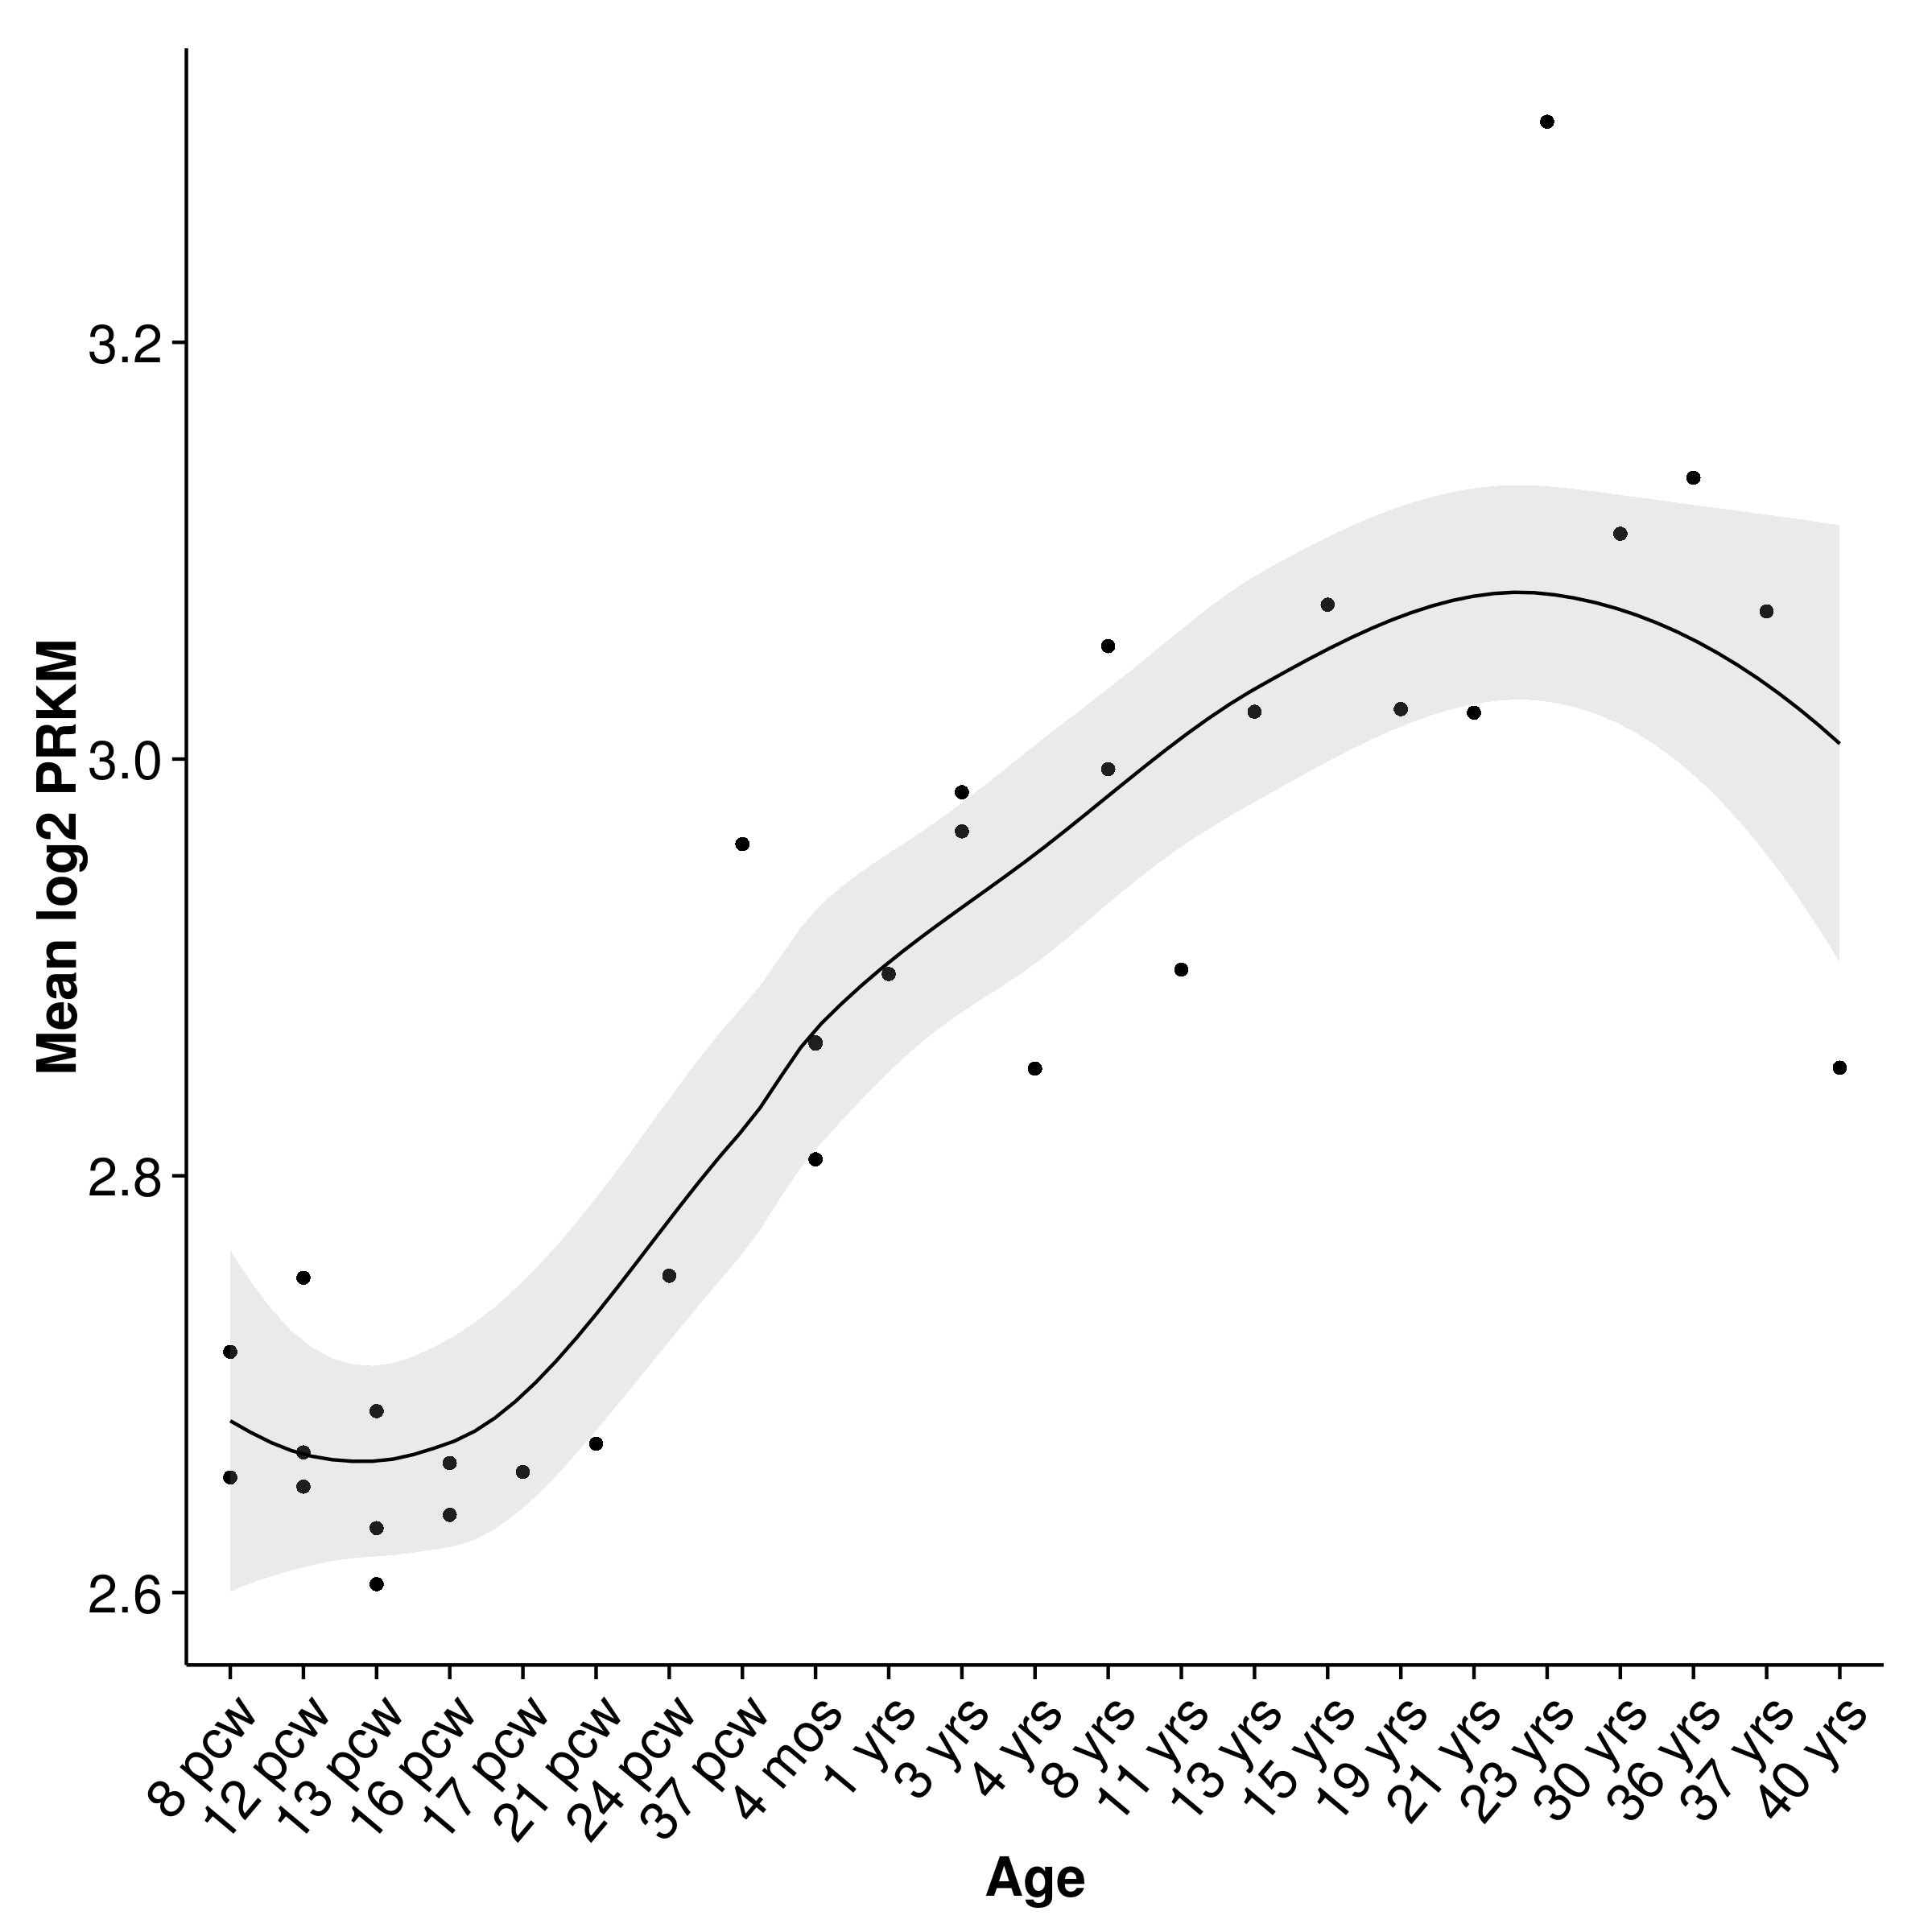
\includegraphics{figure/network/amy_tan_network}}
		\label{fig:tanMod}
	}\\
	\subfloat[``Pink'' Network from Amygdala]{
		\scalebox{.4}{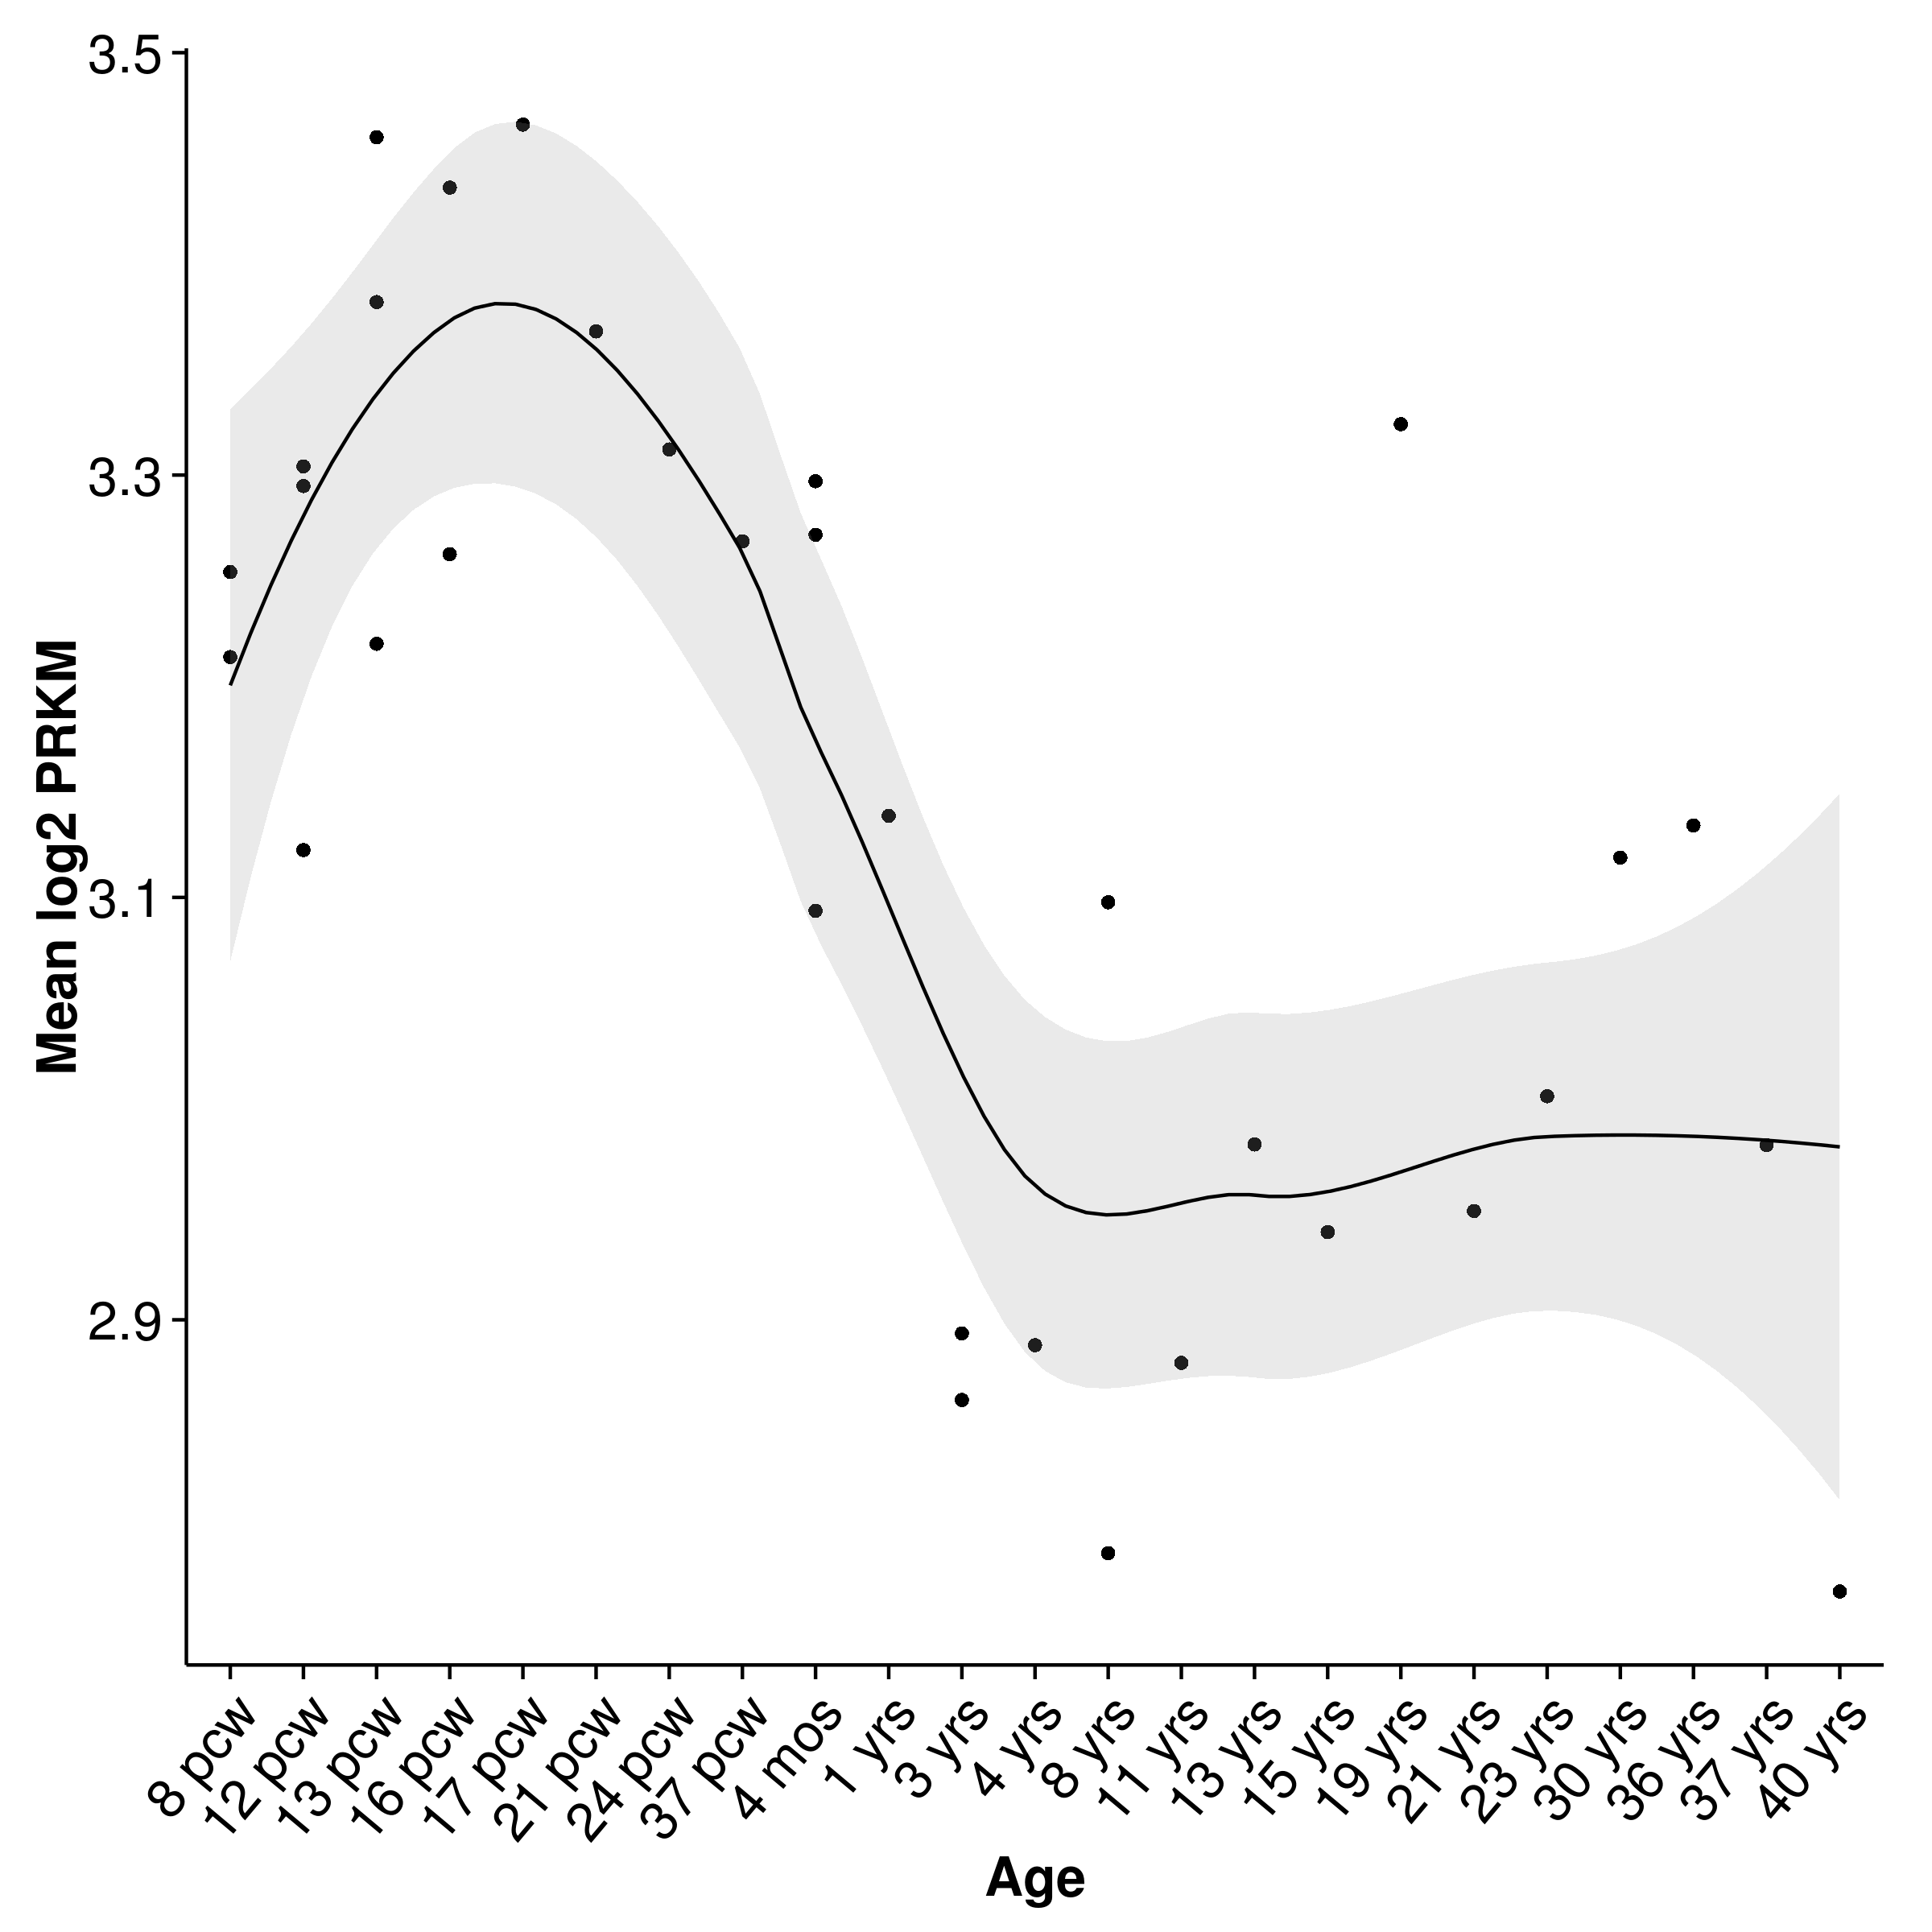
\includegraphics{figure/network/amy_pink_network}}
		\label{fig:pinkMod}
	}
	\subfloat[``Yellow'' Network from Amygdala]{
		\scalebox{.4}{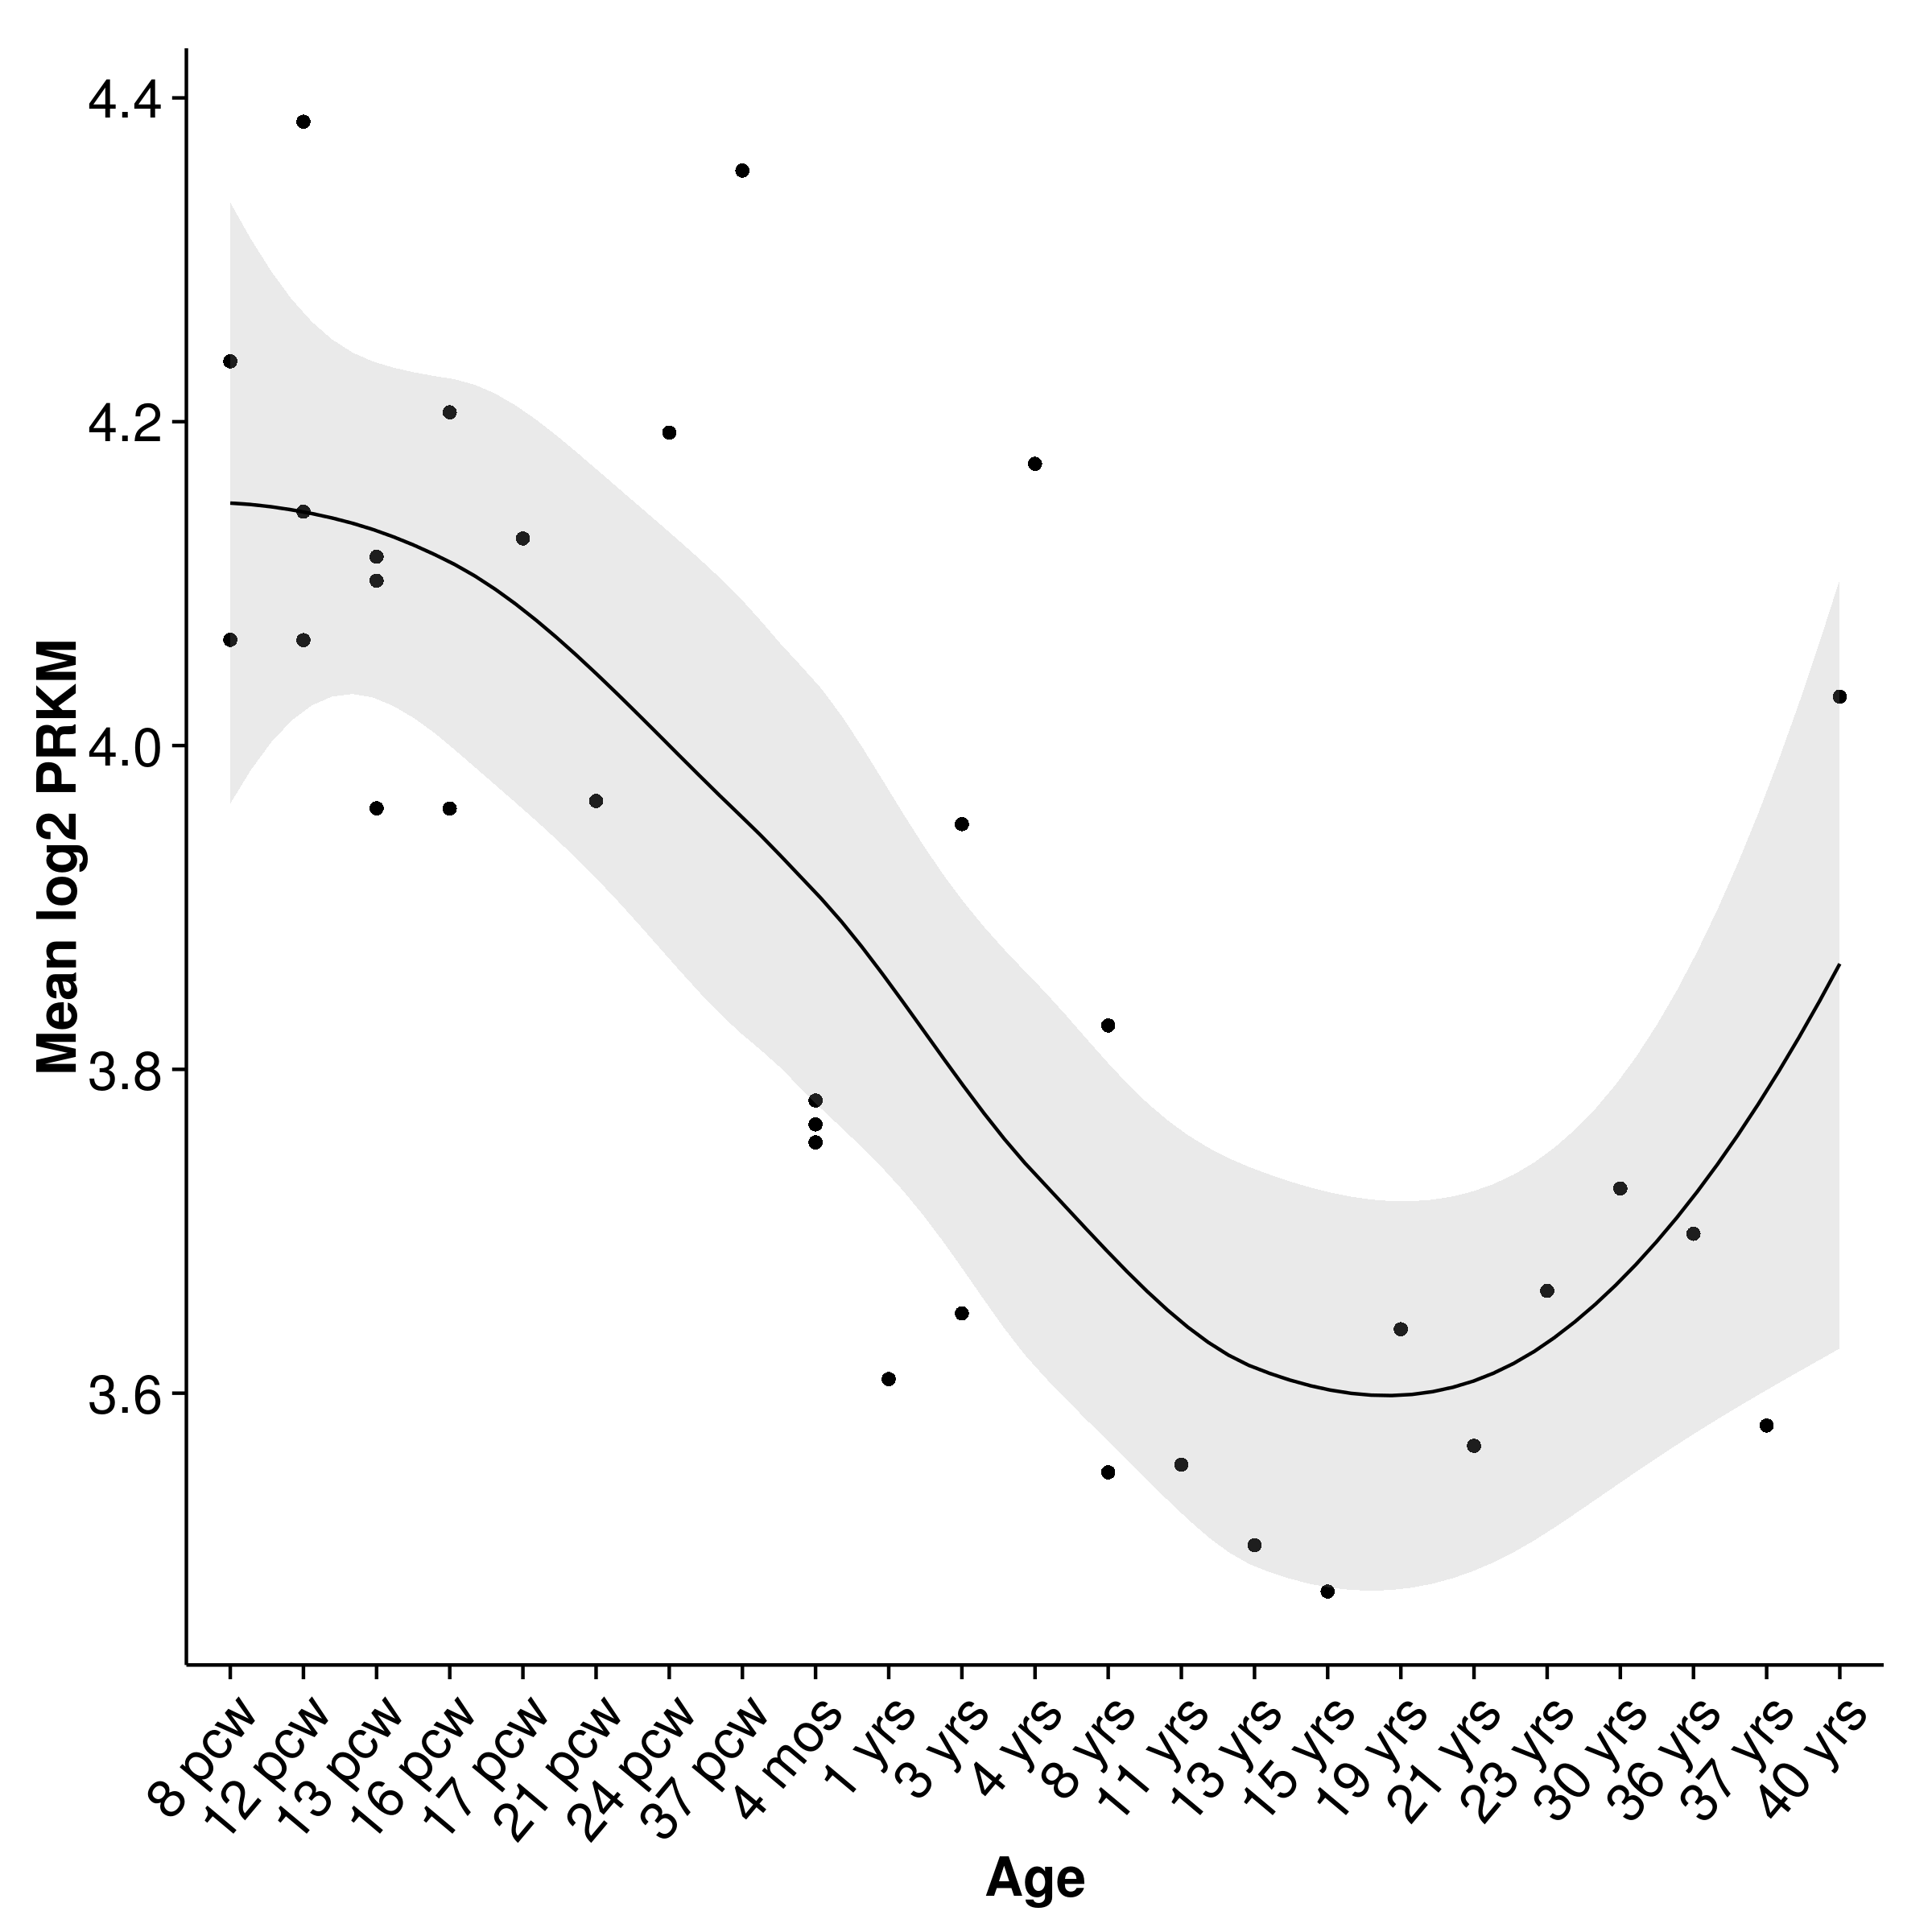
\includegraphics{figure/network/amy_yellow_network}}
		\label{fig:yellowMod}
	}
	\label{fig:allMod}
\end{figure}



\subsubsection{Functional Annotation}
Upon performing the \gls{GO} enrichment analysis, a total of 16 \gls{GO} terms were enriched in the ``black'' hippocampus network, 4 in the ``tan'' amygdala network and 45 in the ``yellow'' amygdala network. 
No \gls{GO} term was enriched in the ``pink'' amygdala network.

The enriched \gls{GO} terms of the ``yellow'' amygdala network were mainly related to translation and transcription and were not specific to brain function or development(\cref{tab:yellowGO}). 
On the contrary, the \gls{GO} terms enriched in the ``black'' hippocampus network were highly relevant to brain function and development (\cref{tab:blackGO})(e.g. ``central nervous system development'' and ``glutamate metabolic process'') and the ``tan'' amygdala network were also related to ammonium ion metabolism (\cref{tab:tanGO}) which is vita for glutamine synthesis from glutamate\citep{Liaw1995}. 

Together, it is highly likely that the ``black'' hippocampus and ``tan'' amygdala networks are related to brain development and function.

\begin{table}[h]
	\centering
	\caption[\glsentryshort{GO} enrichment results for the ``black'' network from Hippocampus]{\gls{GO} enrichment results for the ``black'' network from Hippocampus.
		Among the enriched \gls{GO} terms, it was most interesting to identify a number of brain developmental related \gls{GO} terms such as ``central nervous system development'', ``axon ensheathment in central nervous system'', ``glutamate metabolic process'' and ``positive regulation of gliogenesis''. 
		Surprisingly, \gls{GO} related to immune systems were also observed ``positive regulation of production of molecular mediator of immune response''.
	}
	\begin{tabular}{rrr}
		\toprule
		term\_ID & description & p-value \\
		\midrule
		GO:0019752 & carboxylic acid metabolic process & $4.92\times 10^{-6}$ \\
		GO:0007417 & central nervous system development & $5.94\times 10^{-5}$ \\
		GO:0002821 & positive regulation of adaptive immune response & $6.12\times 10^{-5}$ \\
		GO:0006082 & organic acid metabolic process & $1.03\times 10^{-3}$ \\
		GO:0032291 & axon ensheathment in central nervous system & $1.86\times 10^{-3}$ \\
		GO:1901565 & organonitrogen compound catabolic process & $1.99\times 10^{-3}$ \\
		GO:0006536 & glutamate metabolic process & $3.54\times 10^{-3}$ \\
		GO:0021762 & substantia nigra development & $3.73\times 10^{-3}$ \\
		GO:0044281 & small molecule metabolic process & $4.34\times 10^{-3}$ \\
		GO:0030194 & positive regulation of blood coagulation & $4.59\times 10^{-3}$ \\
		GO:0009607 & response to biotic stimulus & $6.14\times 10^{-3}$ \\
		GO:0002702 & positive regulation of production of molecular mediator of immune response & $6.21\times 10^{-3}$ \\
		GO:0034103 & regulation of tissue remodeling & $6.21\times 10^{-3}$ \\
		GO:0014015 & positive regulation of gliogenesis & $7.47\times 10^{-3}$ \\
		GO:0098542 & defense response to other organism & $7.95\times 10^{-3}$ \\
		GO:0019835 & cytolysis & $8.72\times 10^{-3}$ \\
		\bottomrule
	\end{tabular}%
	\label{tab:blackGO}%
\end{table}%
\begin{table}[h]
	\centering
	\caption[\glsentryshort{GO} enrichment results for the ``tan'' network from Amygdala]{\gls{GO} enrichment results for the ``tan'' network from Amygdala.
		Unlike the ``black'' network, only a small number of \gls{GO} terms were enriched. 
		However, these \gls{GO} terms are relatively specific to amine/ammonium ion metabolism.
		Interestingly, ammonium ion are essential to the synthesis of glutamine from glutamate, suggesting that this network might be relate to the glutamate system.
	}
	\begin{tabular}{rrr}
		\toprule
		term\_ID & description & p-value \\
		\midrule
		GO:0097164 & ammonium ion metabolic process & $1.37\times 10^{-3}$ \\
		GO:0044106 & cellular amine metabolic process & $4.2\times 10^{-3}$ \\
		GO:0009308 & amine metabolic process & $5.41\times 10^{-3}$ \\
		GO:0046519 & sphingoid metabolic process & $6.01\times 10^{-3}$ \\
		\bottomrule
	\end{tabular}%
	\label{tab:tanGO}%
\end{table}%

\subsubsection{Associate Co-expression network with \glsentryshort{pgc} schizophrenia data}
Although the co-expression network were extremely interesting for their expression pattern and functional enrichment in brain development and function related \gls{GO} terms, there were no evidence of their involvement nor importance in schizophrenia.
Therefore it is of particular interest for us to test whether if genes within these co-expression networks were associated withs schizophrenia. 

First, gene base p-value of 18,622 genes were calculated using p-values from the \gls{pgc} schizophrenia working group\citep{Ripke2014}.
Gene set enrichment analysis were then performed using \gls{MAGMA}\citep{DeLeeuw2015} to test whether if there genes within the ``black'' hippocampus and ``tan'' amygdala networks were significantly associated with schizophrenia.

Based on the self-contained gene set enrichment analysis, genes within both networks were significantly associated with schizophrenia with p-value of $1.38\times 10^{-41}$ for the ``tan'' amygdala network and $2.70\times 10{-74}$ for the ``black'' hippocampus network.
These suggest that these networks might be disrupted in schizophrenia patients.
%Network	Size	self-contained	competitive
%Amygdala        289   1.3869e-41      0.44715
%Hippocampus     458   2.6993e-74      0.20002




\subsubsection{Partitioning of Heritability}

\section{Discussion}